\chapter{Methodology}

\section{Dataset}
In respect with this thesis, material is required for achieving, files with customer data for reviews is derived products from the Amazon.com are being used. Files mentioned above are collected by Julian McAuley, Researcher, University of California, and is available on website: http://jmcauley.ucsd.edu/data/amazon/.

The files were extracted from the compressed json format into json files which had users with atleast 5 reviews each (5-core). The duplicates found in the dataset were removed, less than 1 percent of reviews.

The dataset contained product reviews spanning May 1996 - July 2014. Each product review is provided with the following labels:
\begin{itemize}
\item reviewerID: the ID of the reviewer
\item asin: \textit{Amazon Standard Identification Number} given to specific amazon listed item being reviewed
\item reviewerName: the name of the reviewer
\item helpful: how useful the rating \& the review were to some fraction to users
\item reviewText: the textual review left by the reviewer on a specific product
\item overall: product rating by specific reviewer on the item
\item summary: the review summary
\item unixReviewTime: time of the review (unix time)
\item reviewTime: time of the review in mm/dd/yyyy
\end{itemize}

\textbf{Sample review} from the dataset:
\begin{verbatim}
  {
    "reviewerID": "AWY3EPKEOUV1W", 
    "asin": "5555991584", 
    "reviewerName": "Heather", 
    "helpful": [2, 3], 
    "reviewText": "I just recently purchased her ''Paint The Sky With Stars''
    CD and was so impressed that I bought 3 of her previously released CD's and
    plan to buy all her music.  She is truely talented and her music is very
    unique with a combination of modern classical and pop with a hint of an
    Angelic tone. I still recommend you buy this CD. Anybody who has an
    appreciation for music will certainly enjoy her music.",
    "overall": 5.0, 
    "summary": "New Enya Fan.  Simply beautiful.", 
    "unixReviewTime": 978393600, 
    "reviewTime": "01 2, 2001"
  }
\end{verbatim}

From these labels, we extracted the following columns for analysis:
\begin{itemize}
	\item asin: the product ID of the item being reviewed
	\item reviewText: the text review
	\item overall: the corresponding overall rating of the text review
	\item reviewerID: the amazon user id of the user who posted the review
\end{itemize}

The remaining elements were considered irrelevant in the scope of this thesis work, as our work mostly focuses on creating Rating Matrix, Document-term Matrix, and other matrices. This data was retrieved from the json files with the help of Python programming language.

The amazon dataset contains the product reviews that are categorized in the many categories. In the framework of this thesis, we have decided to analyse two specific dataset categories: Digital Music and Health \& Personal Care. These categories were chosen to justify the two yet broad themes in the recommender systems: Experience products and Search Products. 

Experience products can be defined as products whose quality is difficult to evaluate as it largely depends upon the taste of the different customers. With these kinds of products the user has to buy the product, test it, to form an opinion of the product and thereby evaluating the product to write a review about it. Digital Music was the appropriate fit for this category.

While, search products are products that can be objectively evaluated through key characteristics. This characteristic information can be taken from the website itself, user may not need to buy the product to test it. For this theme of the recommender system, we found that Health \& Personal Care section has the features to justify the product being bought as the user needs information, i.e. ingredients, dosage size, direction of use, etc.

To end, the size of both the datasets was large with upto 230,000 reviews for the largest one. An additional step was performed to \textbf{manage the dataset} to a resonable size. The dataset was reduced to 10,000 product reviews that have been randomly sampled from the original dataset. This was essentially done to perform the experiments and test the hypothesis efficiently.


\begin{figure}[H]
  {\centering {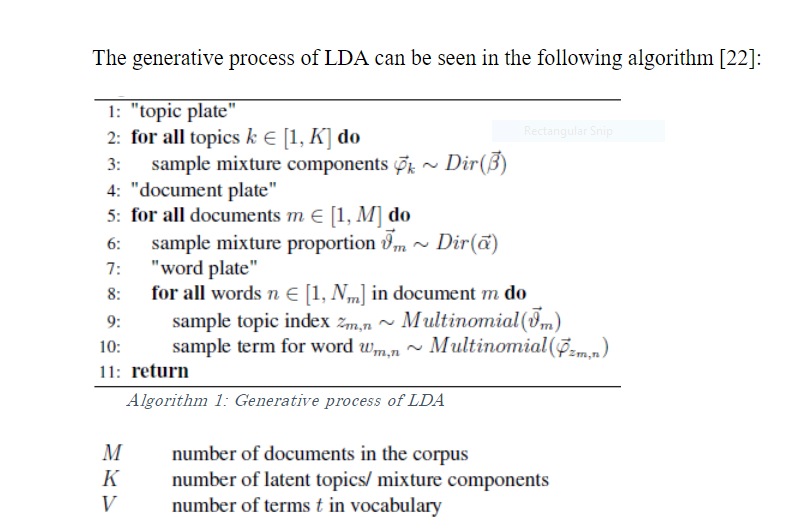
\includegraphics[width = 0.7 \textwidth]{img/lda-formula.png}}\par}
  \caption{LDA algorithm}
\end{figure}


\subsection{Choice of Hyperparameters/Variables Explained}

Use of RMSE value is justified by the previous findings in the study by Koren \cite{Koren2010} \cite{Koren2008} that small improvements in RMSE terms can have significant impact on the quality of some of the top recommendations.

\section{Experiments}
In the course of this thesis, many methods were tried and tested for the recommender systems. Many of them were done on the different datasets, but for the sake of a complete experiment with amazon dataset of the two categories decided as we have seen in the previous section.

\subsection{Approach}
In order to comprehensively describe the experiments made for thesis, a small application of the whole datasets has been implemented which will be fitting the models on the described datasets and evaluate each model on the accuracy basis, and thereafter write the results to the file for the record. The fitting is done using a \textit{4-fold cross validation} mechanism to balance the bad areas of the dataset with longer execution time. Moreover, various values are tried and tested to find the values that are suited best for the better results. 


\begin{figure}
  {\centering {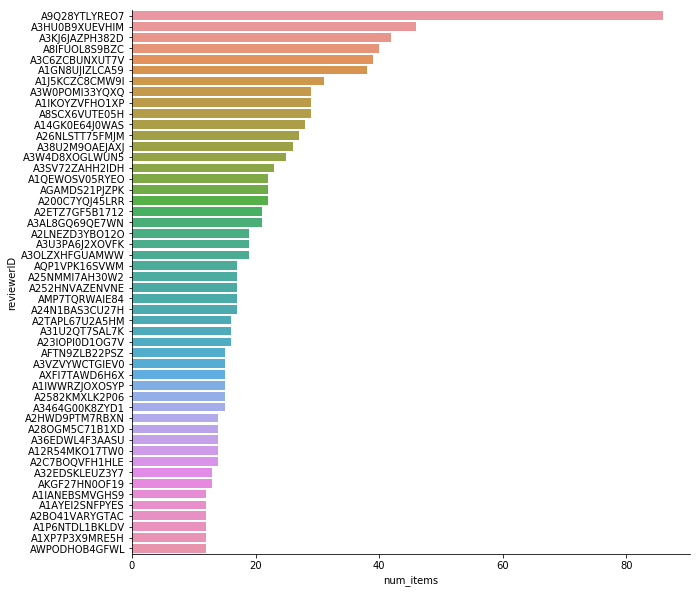
\includegraphics[width = \textwidth]{img/dataset/ItemPerUser50.png}}\par}
\end{figure}



\begin{figure}
  {\centering {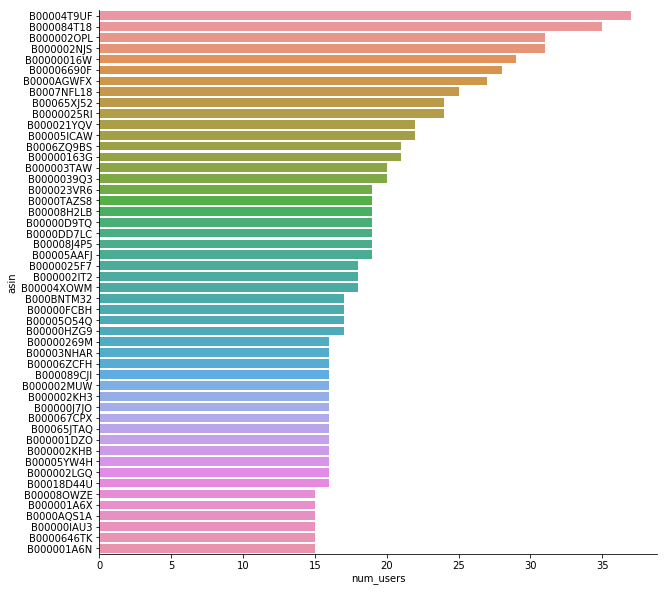
\includegraphics[width = \textwidth]{img/dataset/UserPerItem50.png}}\par}
\end{figure}


\subsection{Implemention}
For implementing the Probabilistic Matrix Factorization and Topic Modelling using Latent Dirichlet Allocation, we used GraphLab - Scientific Library for Python, and also implemented Gibbs Sampling technique.

Graphs were designed using the statistical data visualization python library "\textit{seaborn}"[30].

\subsection{Models}
Using GraphLab python API, we applied SVD on the recommender factorization model and Topic Model classes on two datasets separately. This yielded us with thorough details about the model fitted and evaluated. Models were trained with much of their default settings and some manually optimized hyperparameters and a variable rank. The results generated from the models are then written to the text file and later visualized through plotting.

\subsubsection{Matrix Factorization Model}
FactorizationRecommender trains a model capable of predicting a score for each possible combination of users and items. The internal coefficients of the model are learned from known scores of users and items. Recommendations are then based on these scores.

In the two factorization models, users and items are represented by weights and factors. These model coefficients are learned during training. Roughly speaking, the weights, or bias terms, account for a user or item’s bias towards higher or lower ratings. For example, an item that is consistently rated highly would have a higher weight coefficient associated with them. Similarly, an item that consistently receives below average ratings would have a lower weight coefficient to account for this bias.

The factor terms model interactions between users and items. For example, if a user tends to love romance movies and hate action movies, the factor terms attempt to capture that, causing the model to predict lower scores for action movies and higher scores for romance movies. Learning good weights and factors is controlled by several options outlined below.

\[
  \operatorname{score}(i, j) = \mu + w_i + w_j + \mathbf{a}^T \mathbf{x}_i + \mathbf{b}^T \mathbf{y}_j + {\mathbf u}_i^T {\mathbf v}_j
  \]

where μ is a global bias term, wi is the weight term for user i, wj is the weight term for item j, xi and yj are respectively the user and item side feature vectors, and a and b are respectively the weight vectors for those side features. The latent factors, which are vectors of length numfactors, are given by ui and vj.

\subsubsection{Topic Modelling}

A topic model assumes each document is a mixture of a set of topics, where for each topic some words are more likely than others. One statistical approach to do this is called a “topic model”. This method learns a topic model for the given document collection.

With plate notation, which is often used to represent probabilistic graphical models (PGMs), the dependencies among the many variables can be captured concisely. The boxes are "plates" representing replicates, which are repeated entities. The outer plate represents documents, while the inner plate represents the repeated word positions in a given document, each of which position is associated with a choice of topic and word. M denotes the number of documents, N the number of words in a document. The variable names are defined as follows:

$\alpha$ is the parameter of the Dirichlet prior on the per-document topic distributions,\\
$\beta$ is the parameter of the Dirichlet prior on the per-topic word distribution,\\
\[{\theta_{m}}\] is the topic distribution for document m,\\
$\varphi_{k}$ is the word distribution for topic k,\\
$z_{mn}$ is the topic for the n-th word in documenxt m, and \\
$w_{mn}$ is the specific word.


In order to actually infer the topics in a corpus, we imagine a generative process whereby the documents are created, so that we may infer, or reverse engineer, it. We imagine the generative process as follows. Documents are represented as random mixtures over latent topics, where each topic is characterized by a distribution over all the words. LDA assumes the following generative process for a corpus $D$ consisting of $M$ documents each of length $N_{i}$:

1. Choose $\theta _{i}(\alpha ) \theta _{i} (\alpha)$, where $i\in \{1,\dots ,M\}$ and ($\alpha$ ) is a Dirichlet distribution with a symmetric parameter $\alpha$ which typically is sparse $\alpha$ < 1.

2. Choose $\varphi _{k}$ {Dir} ($\beta$) $\varphi _{k} \beta$, where $k\in \{1,\dots ,K\}$ and $\beta$ typically is sparse

3. For each of the word positions $i,j$, where $i\in \{1,\dots ,M\}$, and $j\in \{1,\dots ,N_{i}\}$. \\

(a) Choose a topic $z_{i,j}$ $\theta_{i}$.\\
(b) Choose a word $w_i,j$ $\varphi_{z_{i,j}} w_{i,j}$ $varphi _{z_{i,j}}$.
(Note that multinomial distribution here refers to the multinomial with only one trial, which is also known as the categorical distribution.)

The lengths $N_{i}$ are treated as independent of all the other data generating variables ($w$ and $z$). The subscript is often dropped, as in the plate diagrams shown here.


